\documentclass{scrreprt}
\usepackage{listings}
\usepackage{underscore}
\usepackage{ragged2e}
\usepackage[bookmarks=true]{hyperref}
\usepackage[utf8]{inputenc}
\usepackage[english]{babel}
\usepackage{xcolor}
\usepackage{amsmath,amssymb}
\usepackage{indentfirst}
\usepackage[section]{placeins}
\usepackage{graphicx}
\usepackage{graphics}
\usepackage{longtable}
\usepackage{booktabs}
\usepackage{xcolor} % for different colour comments
\usepackage{tabto}
\usepackage{array}
\usepackage{mdframed}
\mdfsetup{nobreak=true}
\usepackage{xkeyval}
\usepackage{tabularx}
\hypersetup{
    colorlinks,
    citecolor=black,
    filecolor=black,
    linkcolor=red,
    urlcolor=blue
}
\usepackage[skip=2pt, labelfont=bf]{caption}
\usepackage{titlesec}
\usepackage{float}
\graphicspath{ {image/} }

\titleformat{\paragraph}
{\normalfont\normalsize\textbfseries}{\theparagraph}{1em}{}
\titlespacing*{\paragraph}
{0pt}{3.25ex plus 1ex minus .2ex}{1.5ex plus .2ex}


%% Comments
\newif\ifcomments\commentstrue

\ifcomments
\newcommand{\authornote}[3]{\textcolor{#1}{[#3 ---#2]}}
\newcommand{\todo}[1]{\textcolor{red}{[TODO: #1]}}
\else
\newcommand{\authornote}[3]{}
\newcommand{\todo}[1]{}
\fi

\newcommand{\wss}[1]{\authornote{magenta}{SS}{#1}}
\newcommand{\ds}[1]{\authornote{blue}{DS}{#1}}

\begin{document}
\title{\textbf Text to Motion Database\\[\baselineskip]\Large Test Report}
\author{Brendan Duke\\Andrew Kohnen\\Udip Patel\\David Pitkanen\\Jordan Viveiros}
\date{\today}

\maketitle
\tableofcontents
% \listoftables
% \listoffigures
\newpage

\pagenumbering{arabic}


\chapter{Preface}
\section{Revision History}
\begin{table}[H]
\caption{\textbf Revision History}
\begin{tabularx}{\textwidth}{p{3.5cm}p{2cm}X}
\toprule {\textbf Date} & {\textbf Version} & {\textbf Notes}\\
\midrule
March 14, 2017 & 0.0 & File created\\
March 23, 2017 & 0.1 & Initial template completed \\
March 26, 2017 & 0.2 & Completed tables and organized sections\\
April 7, 2017 & 1.0 & Added more detail to tests and tables\\
April 9, 2017 & 1.1 & Added automated testing and PCKh figure. Final documentation revision. \\
\bottomrule
\end{tabularx}
\end{table}
\section{List of Figures}
This document contains one figure located within automated testing, labeled 7.1.
\listoftables

\chapter{Introduction}

\section{Purpose of Document}

The purpose of this manuscript is to document the testing that has been
performed on the Text-to-Motion Database. The testing that has been
performed largely follows the test plan and requirements that were provided in the Test Plan and Software Requirements and Specification documents respectively.

\section{Scope of Testing}

Following good design principles, the Text-To-Motion Database has been modularized into $3$ conceptual modules.  The first module is a web framework that allows users to access key features like uploading media, viewing previous uploads, and running pose estimation through our deep learning algorithm. The database is the second module in the application and is used to store events from the website like account registration or the uploading of new media. The third module is the most expansive and is the deep learning module that is responsible for running pose estimation on a remote server.

Following the application's modular decomposition, the tests have been separated into $3$ conceptual tests and automated testing.

The first stage of testing is the minimum viable product, and was done to ensure that a base level of functionality was provided. This is where we test to see that all of the software modules have been created and can function synchronously. In order to ensure a minimum viable product was complete both system and unit testing were utilized.

The second set of tests focused on Solution Constraints testing or Functional tests.  In this set of tests, the performance of the deep learning algorithm was rigorously tested and quantified. Building upon the testing of the deep learning algorithm the database was tested to ensure the search capabilities by using specific parameters and test cases.

In the third set of tests, volunteers were asked to test the Non-Functional requirements of the finished product. Examples of these requirements include: usability, design requirements and learnability.

The final set of tests were automated tests ran on the http-server in order to verify the server was posting the correct GET and POST calls. These tests were also used to verify the correctness of the pose estimation of an image.

The final section in this document includes a traceability table that helps to organize and explain how tests are connected to the Software Requirements and Specification document.

%I have added a few examples of what the tables should be.
\chapter{Preliminary Testing}

\section{Minimum Viable Product}
%An example of non functional requirements. In test cases where we we want an average we add an additional cell in bold
\subsection{TextToMotion Availability}

\subsubsection{Description}

This test is done to ensure that the TextToMotion Database (brendanduke.ca/) is functioning as intended and available to the public. These tests will be done by first accessing the home page of brendanduke.ca/, and then navigating to other pages within the website. If the pages are available and contain functioning hyperlinks the test will be considered a pass.

\subsubsection{Results}

The website was accessible through the browser at brendanduke.ca with all buttons, URL's, and hyperlinks being responsive the test has been passed.

\begin{table}[H]
        \centering
        \begin{tabular}[t]{||p{0.75cm}|p{4cm}|p{2.5cm}|p{3cm}|p{2.5cm}|p{1cm}||}
                \hline
                \textbf Test \# & \textbf Test & \textbf Initial State & \textbf Expected Output & \textbf Actual Output & \textbf Result\\
                \hline\hline
                3.1 & Input brendanduke.ca to view the home page & Google.ca & The home page of brendanduke.ca & The home page of brendanduke.ca & Pass \\
                \hline
                3.2 & Add ../Account/Register to the URL or click "Register" & brendanduke.ca & The user registration page & The user registration page & Pass \\
                \hline
                3.3 & Add ../Account/Login to the current URL or click "Login" & brendanduke.ca & The user sign in page & The user sign in page & Pass \\
                \hline
                3.4 & Add ../ImagePoseDraw to the current URL or click "ImagePoseDraw" & brendanduke.ca & The ImagePoseDraw page & The ImagePoseDraw page & Pass \\
                \hline
                3.5 &  Add ../Demo to the current URL or click "Demo" & brendanduke.ca & The Demo page with the camera feed & The Demo page with the camera feed & Pass \\
                \hline
                3.6 &  Add ../TextToMotion to the current URL or click "TextToMotion" & brendanduke.ca & The TextToMotion page & The TextToMotion page & Pass \\
                \hline
        \end{tabular}
\end{table}

\subsection{Updating the database}
\subsubsection{Description}

The database allows users to upload images to the database through the website through brendanduke.ca/ImagePoseDraw. The test will be considered a pass if an image can be uploaded successfully and the user lands on ImagePoseDraw without error.

\subsubsection{Input Data}

Throughout this section the input data is referred to by "Input".jpeg and the website location is referenced through ../ImagePoseDraw which represents brendanduke.ca/ImagePoseDraw.

\begin{table}[H]
        \centering
        \begin{tabular}{p{3cm}p{6cm}}
                \hline\hline
                Input & Description\\
                \hline\hline
                AverageGuy.jpg &  A picture of a man standing still and facing the camera\\ %fill in these entries once we have them
                \hline
                AverageGirl.jpg &  A picture of a woman standing still and facing the camera\\ %fill in these entries once we have them
                \hline
                TomBrady.jpg &  A picture of football star Tom Brady\\ %fill in these entries once we have them
                \hline
        \end{tabular}
\end{table}

\subsubsection{Results}

All images uploaded without error and the user was redirected back to brendanduke.ca/ImagePoseDraw after each upload, therefor the test has been passed.

\begin{table}[H]
        \centering
        \begin{tabular}[t]{||p{0.75cm}|p{4cm}|p{2.5cm}|p{3cm}|p{2.5cm}|p{1cm}||}
                \hline
                \textbf Test \# & \textbf Test & \textbf Initial State & \textbf Expected Output & \textbf Actual Output & \textbf Result\\
                \hline\hline
                3.6 & Upload TomBrady.jpeg using the ImagePoseDraw functionality & .. /ImagePoseDraw/Create & Land on ../ImagePoseDraw & Landed on ../ImagePoseDraw & Pass\\
                \hline
                3.7 & Upload AverageGirl.jpeg using the ImagePoseDraw functionality & .. /ImagePoseDraw/Create & Land on ../ImagePoseDraw & Landed on ../ImagePoseDraw & Pass\\
                \hline
                3.8 & Upload AverageGuy.jpeg using the ImagePoseDraw functionality & .. /ImagePoseDraw/Create & Land on ../ImagePoseDraw & Landed on ../ImagePoseDraw & Pass\\
                \hline
        \end{tabular}
\end{table}

\subsection{Verifying Pose Estimation}
\subsubsection{Description}

After the user has uploaded an image for pose estimation they should be able to view the pose estimation that has been run on the image. In order to verify that some form of pose estimation has been run on the image the user must view their upload and have visible annotations made to the image to be considered a pass.

An image once uploaded can be found within brendanduke.ca/ImagePoseDraw/Details/N, where N represents the number of the uploaded image. This can also be achieved by searching through the uploads.

\subsubsection{Results}

Each uploaded image had pose estimation run sucessfuly and resulted in a new image with a skeleton overlay on the limbs so this test was passed.

\begin{table}[H]
        \centering
        \begin{tabular}[t]{||p{0.75cm}|p{4cm}|p{2.5cm}|p{3cm}|p{2.5cm}|p{1cm}||}
                \hline
                \textbf Test \# & \textbf Test & \textbf Initial State & \textbf Expected Output & \textbf Actual Output & \textbf Result\\
                \hline\hline
                3.9 & View TomBrady.jpeg from ../ImagePoseDraw/Details/30 & .. /ImagePoseDraw & TomBrady.jpeg with pose estimated limbs & TomBrady.jpeg with pose estimated limbs & Pass\\
                \hline
                3.10 & View AvergaeGirl.jpeg from ../ImagePoseDraw/Details/26 & .. /ImagePoseDraw & AvergaeGirl.jpeg with pose estimated limbs &AvergaeGirl.jpeg with pose estimated limbs & Pass\\
                \hline
                 3.11 & View AverageGuy.jpeg from ../ImagePoseDraw/Details/27 & .. /ImagePoseDraw & AverageGuy.jpg with pose estimated limbs & AverageGuy.jpg with pose estimated limbs & Pass\\
                \hline
        \end{tabular}
\end{table}

\subsection{Search by Name or Description}
\subsubsection{Description}

The web interface has the ability to search through the uploaded images and videos based on their name or information within the associated description. The test will be considered a pass if the name is input in the search bar and image is returned.

\subsubsection{Results}

All three tests passed as it was successful to search through the entries and find the upload through an associated name or description.

\begin{table}[H]
        \centering
        \begin{tabular}[t]{||p{0.75cm}|p{4cm}|p{2.5cm}|p{3cm}|p{2.5cm}|p{1cm}||}
                \hline
                \textbf Test \# & \textbf Test & \textbf Initial State & \textbf Expected Output & \textbf Actual Output & \textbf Result\\
                \hline\hline
                3.12 & Input  "Tom" in the search bar within ../ImagePoseDraw & .. /ImagePoseDraw & A list of figured including the Tom Brady image that was uploaded & A single return of the Tom Brady image & Pass\\
                \hline
                3.13 & Input "Average" in the search bar within ../ImagePoseDraw & .. /ImagePoseDraw & A list of results including the AverageGirl image & Two results, one of which was Average Girl & Pass\\
                \hline
                 3.14 & Input "Guy" in the search bar within ../ImagePoseDraw & .. /ImagePoseDraw & A list of results including the AverageGuy image & Two results, one of which was Average Guy & Pass\\
                \hline
        \end{tabular}
\end{table}

\section{Solution Constraints Testing}

\subsection{Deep Learning Methods Test}
\subsubsection{Description}

In order to provide a proper demonstration of the deep learning mechanics that can be associated with pose estimation we will meet with Dr.Taylor to ensure that we are implementing the Bulat et al paper properly. This test will be considered a pass if Dr.Taylor is satisfied with the implementation of the previously mentioned paper.

\subsubsection{Results}

\begin{table}[H]
        \centering
        \begin{tabular}{||p{0.75cm}|p{7.5cm}|p{1cm}||}
                \hline
                \textbf Test \# & \textbf Test & \textbf Result\\
                \hline\hline
                3.15 & Meet with Dr.Taylor in order to verify the integrity of the deep learning implementation within the TextToMotion Database. & Pass\\ %fill in these entries once we have them
                \hline
        \end{tabular}
\end{table}

\subsection{Standard Data Format Test}

\subsubsection{Description}

An automated test that checks if the human pose data used for the project is
standard and compatible with existing software libraries.

\subsubsection{Results}

This test was technically a failure. The data was not converted to a format
compatible with libraries. Instead the data is stored in JSON strings, which is
a standard format, but not compressed as an ideal format such as HDF5 would be.


\chapter{Functional Requirements}

\section{Input Data}

Throughout this section the input data is referred to by "Input".MP4 and the website location is referenced through ../ImagePoseDraw which represents brendanduke.ca/ImagePoseDraw.

\begin{table}[H]
        \centering
        \begin{tabular}{p{3cm}p{6cm}}
                \hline\hline
                Input & Description\\
                \hline\hline
                E9FY2.MP4  &  A short video of a woman eating a sandwich\\
                \hline
                U4XV9.MP4  &  A short video of a man waking up and getting out of bed\\
                \hline
                Z1A0Q.MP4 & A short video of a man sitting on a stool\\
                \hline
        \end{tabular}
\end{table}

\section{Supported Video Encoding Test}

\subsection{Description}

Tests whether the ReadFrames API is able to decode MP4 files. If we are able to run pose estimation on the video, then the ReadFrames API is able to process the frames and the test will be considered a pass.

\subsubsection{Results}

Each test was successful in using the ReadFrames API to decode the MP4 files and run pose estimation so this test has been passed.

\begin{table}[H]
        \centering
        \begin{tabular}[t]{||p{0.75cm}|p{4cm}|p{2.5cm}|p{3cm}|p{2.5cm}|p{1cm}||}
                \hline
                \textbf Test \# & \textbf Test & \textbf Initial State & \textbf Expected Output & \textbf Actual Output & \textbf Result\\
                \hline\hline
                4.1 & Using the ReadFrames API on E9FY2.MP4, to run pose estimation & ReadFrame API & A compiled E9FY2.MP4 that has been pose estimated & E9FY2.MP4 with pose estimation & Pass\\
                \hline
                4.2 & Using the ReadFrames API on U4XV9.MP4, to run pose estimation & ReadFrame API & A compiled U4XV9.MP4 that has been pose estimated & U4XV9.MP4 with pose estimation & Pass\\
                \hline
                4.3 & Using the ReadFrames API on Z1A0Q.MP4, to run pose estimation & ReadFrame API & A compiled Z1A0Q.MP4 that has been pose estimated & Z1A0Q.MP4 with pose estimation & Pass\\
                \hline
        \end{tabular}
\end{table}

\section{Frame Reading Timestamp Accuracy Test}
\subsection{Description}

Tests whether the timestamps on the frames returned by the ReadFrames API match their temporal position in the original video stream. In order for this test to be considered a pass two random timestamps will be verified and if they match it will be considered a success. On a single failed timestamp two new timestamps will be taken until it is a definite failure or success.

\subsection{Results}

All three tests were able to match timestamps to the original video and the test has been passed.

\begin{table}[H]
        \centering
        \begin{tabular}[t]{||p{0.75cm}|p{4cm}|p{2.5cm}|p{3cm}|p{2.5cm}|p{1cm}||}
                \hline
                \textbf Test \# & \textbf Test & \textbf Initial State & \textbf Expected Output & \textbf Actual Output & \textbf Result\\
                \hline\hline
                4.4 & Use the ReadFrames API on E9FY2.MP4, in order to verify the timestamps & ReadFrame API & Matching timestamps at 5 and 7 seconds & Matching timestamps at 5 and 7 seconds & Pass\\
                \hline
                4.5 & Use ReadFrames API on U4XV9.MP4, in order to verify the timestamps match & ReadFrame API & Matching timestamps at 3 and 10 seconds & Matching timestamps at 3 and 10 seconds & Pass\\
                \hline
                4.6 & Use ReadFrames API on Z1A0Q.MP4, in order to verify the timestamps match & ReadFrame API & Matching timestamps at 6 and 11 seconds & Matching timestamps at 6 and 11 seconds  & Pass\\
                \hline
        \end{tabular}
\end{table}

\section{Human Pose Estimation Data Quality Test}
\subsection{Description}

Test to ensure the data quality produced by the human pose estimator component
was acceptable.

A set of Charades videos will be processed by the human pose estimator, and
skeleton animations corresponding to the generated human pose data will be
created (this is a scoped part of the software pipeline). A double-blind test
will be ran, wherein testers will be shown random mixed sets of the skeleton
animations produced by McMaster Text to Motion, together with skeletons from
actual motion capture data coming from CMU'’s motion capture lab. Testers will
indicate whether they think the motion capture data came from actual motion
capture, or from the pose estimation software.

The McMaster Text to motion Results should be guessed as accurate at similar
rates to the Charades tests.

\subsection{Results}

We provide the ratio of Text-to-Motion images guessed as accurate compared to the Charades Images.

\begin{table}[H]
        \centering
        \begin{tabular}{||p{0.75cm}|p{7.5cm}|p{2.5cm}|p{2.5cm}||}
                \hline
                \textbf Test \# & \textbf Test & \textbf Charades/ TextToMotion & \textbf Result\\
                \hline\hline
                4.7 & Nick was shown a set of videos and asked to determine which was generated by the TextToMotion Database &  1/1 & Pass\\
                \hline
                4.8 & Drew was shown a set of videos and asked to determine which was generated by the TextToMotion Database&  7/5  & Pass\\
                \hline
                4.9 & Sarah was shown a set of videos and asked to determine which was generated by the TextToMotion Database& 5/4 & Pass\\
                \hline
        \end{tabular}
\end{table}

\section{Database Output Full Range Coverage Test}
\subsection{Description}

Tests to be sure all entries in the database can be successfully searched for. The previous input data has been renamed in order to specify names and descriptions which can be found below. In order for this test to be considered a pass each uploaded video will need to be found when searching for the name or description given.

\subsection{Input Data}

Throughout this section the input data is referred to by "Input".MP4 and the website location is referenced through ../ImagePoseDraw which represents brendanduke.ca/ImagePoseDraw.

\begin{table}[H]
        \centering
        \begin{tabular}{p{3cm}p{6cm}}
                \hline\hline
                Input & Description\\
                % NEED THE BUILD COMMANDS WITH DESCRIPTIONS
                \hline\hline
                \verb|Waking_Up.mp4| &  Given tags sleeping, boy, man, sleepy, getting up, table\\
                \hline
                \verb|Eating.mp4| &  Given tags sandwich, eating, girl, woman, table\\
                \hline
                \verb|Stool.mp4| &  Given tags man, stool, corner, sitting\\
                \hline
        \end{tabular}
\end{table}

\subsubsection{Results}

The given set of videos appeared in the returned list of videos from the search, so this test has been passed.

\begin{table}[H]
        \centering
        \begin{tabular}[t]{||p{0.75cm}|p{4cm}|p{2.5cm}|p{3cm}|p{2.5cm}|p{0.75cm}||}
                \hline
                \textbf Test \# & \textbf Test & \textbf Initial State & \textbf Expected Output & \textbf Actual Output & \textbf Result\\
                \hline\hline
                4.10 & Search for the Waking_Up.mp4 within ../ImagePoseDraw with keyword "Waking" & .. /ImagePoseDraw & A list of results including Waking_Up.MP4 & A single result of the Waking_up.mp4 & Pass\\
                \hline
                4.11 & Search for the Eating.mp4 within ../ImagePoseDraw with keyword "Eat" & .. /ImagePoseDraw & A list of results including Eating.MP4 & A single result of the Eat.mp4 & Pass\\
                \hline
                4.12 & Search for the Stool.mp4 within ../ImagePoseDraw with keyword "sitting" & .. /ImagePoseDraw & A list of results including Stool.Mp4 & A single result of the Stool.mp4 & Pass\\
                \hline
        \end{tabular}
\end{table}

\section{Database No False Positives}
\subsection{Description}

Tests that the database search does not return any false positives, such as
videos or images that do not contain searched words. The same videos from the
previous test will be used with the same tags. Thus, we will search with tags
other than those provided. If no videos appear, then the test is a success.

\subsubsection{Results}

Using the nonsensical keywords from our input data, no search results were
returned, meaning that the test passed.

\begin{table}[H]
        \centering
        \begin{tabular}[t]{||p{0.75cm}|p{4cm}|p{2.5cm}|p{3cm}|p{2.5cm}|p{0.75cm}||}
                \hline
                \textbf Test \# & \textbf Test & \textbf Initial State & \textbf Expected Output & \textbf Actual Output & \textbf Result\\
                \hline\hline
                4.13 & Search for "Raptor" within ../ImagePoseDraw & .. /ImagePoseDraw & A list of results that don't contain the input data & No results were returned & Pass\\
                \hline
                4.14 & Search for "Exponent" within ../ImagePoseDraw & .. /ImagePoseDraw & A list of results that don't contain the input data & No results were returned & Pass\\
                \hline
                4.15 & Search for "Glasses" within ../ImagePoseDraw & .. /ImagePoseDraw & A list of results that don't contain the input data & No results were returned & Pass\\
                \hline
        \end{tabular}
\end{table}

\section{HTTP GET test}
\subsection{Description}

A test to ensure the HTTP server can receive GET requests with an image, and return a JSON string of values containing joint positions. We present the values as an array, where each vertex has two components representing the x and y position. If every value is between -0.5 and 0.5 then the data returned is accurate, and the test is a pass. The GET requests were created using curl with the -X GET option and attempting to reach brendanduke.ca:8765
\subsection{Input Data}

\begin{table}[H]
        \centering
        \begin{tabular}{p{3cm}p{6cm}}
                \hline\hline
                Input & Description\\
                \hline\hline
                \href {http://st2.depositphotos.com/1912333/10089/i/950/depositphotos_100892946-stock-photo-sporty-woman-waving-hands.jpg}{Sporty Woman} &  A picture of a woman standing and waving her hands\\
                \hline
                \href {https://www.drawingnow.com/file/videos/image/how-to-draw-a-running-person.jpg}{Running Man} & An illustration of a man running\\
                \hline
                \href {https://www.formfonts.com/files/1/13470/four-low-poly-models-people-sitting-different-poses_FF_Model_ID13470_1_LPMAD_20_00.jpg}{Sitting Man} & A 3d model of a person sitting\\
                \hline
        \end{tabular}
\end{table}

\subsection{Results}
\begin{table}[H]
        \centering
        \begin{tabular}[t]{||p{0.75cm}|p{4cm}|p{2.5cm}|p{3cm}|p{2.5cm}|p{1cm}||}
                \hline
                \textbf Test \# & \textbf Test & \textbf Initial State & \textbf Expected Output & \textbf Actual Output & \textbf Result\\
                \hline\hline
                4.16 & Using curl -X GET with parameters of brendenduke.ca:8765 and the Sporty Woman image & CMD line with curl installed & An array of values between -0.5 and 0.5 & See Table 4.1 & Pass\\
                \hline
                4.17 & Using curl -X GET with parameters of brendenduke.ca:8765 and the Running Man image & curl is installed and functional & An array of values between -0.5 and 0.5 & See Table 4.2 & Pass\\
                \hline
                4.18 & Using curl -X GET with parameters of brendenduke.ca:8765 and the Sitting Man image & curl is installed and functional & An array of values between -0.5 and 0.5 & See Table 4.3 & Pass\\
                \hline
        \end{tabular}
\end{table}

\subsection{Output Data}

\begin{table}[H]
    \centering
    \caption{For test 4.16 (r is for left and l is for right)}
    \begin{tabular}{||p{2cm}|p{6.5cm}||}
        \hline
        \textbf{Body Part} & \textbf {JSON Values}\\
         \hline\hline
        r ankle & [-0.0736842105263, 0.328947368421] \\
        \hline
        r knee & [-0.0315789473684, 0.157894736842] \\
        \hline
        r hip & [-0.0526315789474, 0.0105263157895] \\
        \hline
        l hip & [-0.0315789473684, 0.0315789473684] \\
        \hline
        l knee & [-0.0315789473684, 0.157894736842] \\
        \hline
        l ankle & [-0.0315789473684, 0.157894736842] \\
        \hline
        pelvis & [-0.0342105263158, 0.0105263157895]\\
        \hline
        thorax & [-0.0105263157895, -0.223684210526] \\
        \hline
        upper neck & [0.0105263157895, -0.244736842105] \\
        \hline
        head top & [0.0105263157895, -0.394736842105] \\
        \hline
        r wrist & [-0.223684210526, -0.328947368421] \\
        \hline
        r elbow & [-0.202631578947, -0.244736842105] \\
        \hline
        r shoulder & [-0.0526315789474, -0.223684210526] \\
        \hline
        l shoulder & [0.0526315789474, -0.223684210526] \\
        \hline
        l elbow & [0.181578947368, -0.265789473684] \\
        \hline
        l wrist & [0.160526315789, -0.371052631579] \\
        \hline
    \end{tabular}
\end{table}

\begin{table}[H]
    \centering
    \caption{For test 4.17 (r is for left and l is for right)}
    \begin{tabular}{||p{2cm}|p{6.5cm}||}
        \hline
        \textbf{Body Part} & \textbf {JSON Values}\\
         \hline\hline
        r ankle & [-0.157894736842, 0.244736842105] \\
        \hline
        r knee & [-0.0736842105263, 0.0947368421053] \\
        \hline
        r hip & [0.0315789473684, -0.0315789473684] \\
        \hline
        l hip & [0.0315789473684, -0.0526315789474] \\
        \hline
        l knee & [0.0526315789474, 0.118421052632] \\
        \hline
        l ankle & [0.223684210526, 0.0736842105263] \\
        \hline
        pelvis & [0.0315789473684, -0.0342105263158]\\
        \hline
        thorax & [-0.0315789473684, -0.157894736842] \\
        \hline
        upper neck & [-0.0315789473684, -0.157894736842] \\
        \hline
        head top & [-0.0526315789474, -0.328947368421] \\
        \hline
        r wrist & [-0.0105263157895, -0.0315789473684] \\
        \hline
        r elbow & [-0.0315789473684, -0.0736842105263] \\
        \hline
        r shoulder & [-0.0526315789474, -0.157894736842] \\
        \hline
        l shoulder & [-0.0526315789474, -0.160526315789]\\
        \hline
        l elbow & [0.0526315789474, -0.157894736842] \\
        \hline
        l wrist & [0.0526315789474, -0.0315789473684] \\
        \hline
    \end{tabular}
\end{table}

\begin{table}[H]
    \centering
    \caption{For test 4.18 (r is for left and l is for right)}
    \begin{tabular}{||p{2cm}|p{6.5cm}||}
        \hline
        \textbf{Body Part} & \textbf {JSON Values}\\
         \hline\hline
        r ankle & [-0.139473684211, 0.328947368421]\\
        \hline
        r knee & [-0.221052631579, 0.0526315789474]\\
        \hline
        r hip & [-0.0315789473684, -0.0105263157895] \\
        \hline
        l hip & [0.0763157894737, 0.0315789473684] \\
        \hline
        l knee & [-0.0315789473684, 0.202631578947] \\
        \hline
        l ankle & [-0.0736842105263, 0.371052631579]\\
        \hline
        pelvis & [0.0315789473684, 0.0105263157895] \\
        \hline
        thorax & [0.0947368421053, -0.265789473684] \\
        \hline
        upper neck & [0.0763157894737, -0.328947368421] \\
        \hline
        head top & [0.0526315789474, -0.5] \\
        \hline
        r wrist & [-0.118421052632, -0.0736842105263]\\
        \hline
        r elbow & [-0.0736842105263, -0.118421052632]\\
        \hline
        r shoulder & [-0.0105263157895, -0.265789473684] \\
        \hline
        l shoulder & [0.202631578947, -0.244736842105] \\
        \hline
        l elbow & [0.178947368421, -0.0736842105263] \\
        \hline
        l wrist & [0.0315789473684, -0.0552631578947] \\
        \hline
    \end{tabular}
\end{table}

\section{False Positive Test}
\subsection{Description}

Tests whether the HTTP server will return a 404 error when attempting to make an empty GET request. To do this we SSL to the server (openssl s\_client -connect brendanduke.ca:8765) and  when asked for an input, hit enter/return twice to create an empty request.
\subsection{Results}
\begin{table}[H]
        \centering
        \begin{tabular}[t]{||p{0.75cm}|p{2.5cm}|p{2.5cm}|p{3cm}|p{3.5cm}|p{1cm}||}
                \hline
                \textbf Test \# & \textbf Test & \textbf Initial State & \textbf Expected Output & \textbf Actual Output & \textbf Result\\
                \hline\hline
                4.19 & Sending an empty request with SSL & CMD line with curl installed & A 404 Error & HTTP/1.0 400 Bad Request  Server: BaseHTTP/0.6 Python/3.5.2 & Pass\\
                \hline
        \end{tabular}
\end{table}

%For tests that require a time use this
\chapter{Non-Functional Requirements}
\section{Usability}
\subsection{Description}
In order to determine the usability of the Text-to-Motion database, a small
sample of users were asked to use the website to perform some predetermined
actions and answer questions afterwards.

Before the participants were asked to preform any actions they were given a minute to familiarize themselves with the interface, but were not given any guidance or tips from the development team. Once the time was up they were asked to upload an image using their mobile device or desktop. If they used the desktop the user either uploaded an image through a URL or a previously saved file.

While performing the required action the participant's time was recorded and
used to determine if a requirement had passed or failed. Upon completion of the task the users were asked to rate the style and design of the website on a scale from 1 to 10, with 1 being the lowest option and 10 being the highest.

\subsection{Results}

The results from the participants can be seen throughout the Non-Functional
Requirements along with a pass or fail based on the requirements description.

\section{Look and Feel Requirements}
\subsection{Colour Scheme}
\subsubsection{Description}

A test to see if the colour scheme of the website is visually appealing. Making the colour scheme of the website visually appealing to a larger audience is important as it will help keep users on the website and ideally provide a reason to reference it to a friend or colleague.

When testing the colour scheme anything above a 6 was considered a pass. We chose anything above a 6 because with this rating it means users enjoyed the colour scheme and may result in them recommending the website to others or returning.

\subsubsection{Results}

\begin{table}[H]
        \centering
        \begin{tabular}{||p{0.75cm}|p{2.5cm}|p{3cm}|p{2.5cm}|p{2.5cm}||}
                \hline
                \textbf Test \# & \textbf User & \textbf Initial State & \textbf Rating & \textbf Result\\
                \hline\hline
                5.1 & Nick & brendanduke.ca & 7 & Pass \\
                \hline
                5.2 & Drew & brendanduke.ca & 9 & Pass\\ %fill in these entries once we have them
                \hline
                5.3 & Sarah & brendanduke.ca & 7 & Pass \\
                \hline
        \end{tabular}
\end{table}

\section{Style Requirements}

\subsection{Minimalistic Web Design}
\subsubsection{Description}

The website interface should be minimal and should inform the user of valid
actions through visual means. This is a modern requirement in website design, the more minimalistic design you can provide the better it will be for the user experience and any new technologies use to enforce this will help drive traffic.

While testing the minimalistic design anything above a 7 was considered a pass. This required a higher rating then the colour scheme as we believed it would be a key factor in providing the user with an enjoyable experience and help provide a greater amount of uploads if the interface was easily understood.

\subsubsection{Results}

\begin{table}[H]
        \centering
        \begin{tabular}{||p{0.75cm}|p{2.5cm}|p{3cm}|p{2.5cm}|p{2.5cm}||}
                \hline
                \textbf Test \# & \textbf User & \textbf Initial State & \textbf Rating & \textbf Result\\
                \hline\hline
                5.4 & Nick & brendanduke.ca & 9 & Pass \\
                \hline
                5.5 & Drew & brendanduke.ca & 9 & Pass\\ %fill in these entries once we have them
                \hline
                5.6 & Sarah & brendanduke.ca & 8 & Pass \\
                \hline
        \end{tabular}
\end{table}

\section{Ease of Use Requirements}
\subsection{Upload/Download}
\subsubsection{Description}

Through the web interface a user should be able to upload a picture using
either a mobile phone camera, URL, or saved file. The participant will start on
the Home page and be asked to upload an image through one of the methods previously
mentioned.

In order for this to be considered a pass it should take the users 45 seconds or less to complete the upload process and click the button. The required time of 45 seconds was chosen due to the amount of time that was required to find an image, URL, or file  while running trials throughout the development.

\subsubsection{Results}
\begin{table}[H]
        \centering
        \begin{tabular}[t]{||p{0.75cm}|p{4cm}|p{2.5cm}|p{3cm}|p{2.5cm}|p{0.75cm}||}
                \hline
                \textbf Test \# & \textbf Test & \textbf Initial State & \textbf User & \textbf Time & \textbf Result\\
                \hline\hline
                5.7 & Upload an image from a URL & .. /ImagePoseDraw/Create & Nick & 32 seconds & Pass\\
                \hline
                5.8 & Upload an image from a mobile device & .. /ImagePoseDraw/Create & Drew & 38 seconds & Pass\\
                \hline
                5.9 & Upload a file stored within the Desktop & .. /ImagePoseDraw/Create & Sarah & 27 seconds & Pass\\
                \hline
        \end{tabular}
\end{table}

\subsection{Text Box Functionality}
\subsubsection{Description}

The user should be able to input a descriptive word or phrase into a text-box
from within the web interface in order to search for a video. With a the website being part of a larger database the ability to search for an image that the user just uploaded is an important factor in determining the usability for users.

In order to complete this task the users were asked to search for a specific word and
display the results. Any time below 10 seconds will be considered a pass. Each user was allocated 10 seconds because we did not want the action of typing the keyword to be the bottleneck when searching for a database entry.

\subsubsection{Results}
\begin{table}[H]
        \centering
        \begin{tabular}[t]{||p{0.75cm}|p{4cm}|p{2.5cm}|p{3cm}|p{2.5cm}|p{0.75cm}||}
                \hline
                \textbf Test \# & \textbf Test & \textbf Initial State & \textbf User & \textbf Time & \textbf Result\\
                \hline\hline
                5.10 & Search for "Woman" & .. /ImagePoseDraw & Nick & 4 seconds & Pass\\
                \hline
                5.11 & Search for "f" & .. /ImagePoseDraw & Drew & 3 seconds & Pass\\
                \hline
                5.12 & Saerch for "the" & .. /ImagePoseDraw & Sarah & 4 seconds & Pass\\
                \hline
        \end{tabular}
\end{table}

\section{Learning Requirements}

\subsection{Usability Tests}
\subsubsection{Description}

The user should be able to interact with the website without any previous knowledge.
They will given a minute to explore the website. After that time the
participants were asked to rate the usability on a scale of 1-10.

In order for the result to be considered a pass the ranking must be greater then a 6. This was chosen as having a website that is usable to someone without any prior knowledge to pose estimation or deep learning keeps the users that may use the website much larger and widely accepted.

\subsubsection{Results}

\begin{table}[H]
        \centering
        \begin{tabular}{||p{0.75cm}|p{2.5cm}|p{2.5cm}|p{2.5cm}||}
                \hline
                \textbf Test \# & \textbf User & \textbf Rating & \textbf Result\\
                \hline\hline
                5.13 & Nick & 7 & Pass \\
                \hline
                5.14 & Drew & 8 & Pass\\ %fill in these entries once we have them
                \hline
                5.16 & Sarah & 7 & Pass \\
                \hline
        \end{tabular}
\end{table}

\section{Politeness and Understandability Requirements}
\subsection{Hiding the Inner Workings}
\subsubsection{Description}

Users should not be able to see the deep learning model and its training when
using the pose estimation. When prompted the website should display the correct
skeletons without any low-level detail. Once the image was uploaded the participants were asked if they saw anything that seemed out of place or any information on the software used, if they did not it will be considered a pass.

\subsubsection{Results}

Users indicated that the deep learning model was encapsulated from their view,
and hence this test passed.

\begin{table}[H]
        \centering
        \begin{tabular}[t]{||p{0.75cm}|p{4cm}|p{2.5cm}|p{3cm}|p{2.5cm}|p{0.75cm}||}
                \hline
                \textbf Test \# & \textbf Test & \textbf Initial State & \textbf User  & \textbf Result\\
                \hline\hline
                5.17 & Uploading an image from URL & .. /ImagePoseDraw/Create & Nick & Pass\\
                \hline
                5.18 & Uploading an image from mobile & .. /ImagePoseDraw/Create & Drew & Pass\\
                \hline
                5.19 & Uploading an image from desktop & .. /ImagePoseDraw/Create & Sarah & Pass\\
                \hline
        \end{tabular}
\end{table}

\section{Speed and Latency Testing}

\subsection{External Database Connection and Verification Time}
\subsubsection{Description}

The web interface should be able to connect to an external database and store
or query items. In order for this test to be considered a pass the confirmation
of the image being uploaded would have to occur within 60 seconds so that
additional resources are not wasted by the database.

The required time was determined to be 60 seconds because we are remotely connecting to a server within the University of Guelph in order to access their GPU and would add time to the total execution time.

\subsubsection{Input Data}

\begin{table}[H]
        \centering
        \begin{tabular}{p{3cm}p{6cm}}
                \hline\hline
                Input & Description\\
                % NEED THE BUILD COMMANDS WITH DESCRIPTIONS
                \hline\hline
                URL image & An image of a male  \\
                \hline\hline
                Desktop file & An image of Seth Rogan \\
                \hline\hline
                Mobile image & An image of Andrew \\
                \hline
        \end{tabular}
\end{table}

\subsubsection{Results}

According to the response times of this test and verification, the database queries
were executed fast enough for the test to pass.

\begin{table}[H]
        \centering
        \begin{tabular}[t]{||p{0.75cm}|p{3cm}|p{2.5cm}|p{2.5cm}|p{2.5cm}|p{1cm}|p{1cm}||}
                \hline
                \textbf Test \# & \textbf Test & \textbf Initial State & \textbf Expected State & \textbf Actual State &\textbf Time & \textbf Result\\
                \hline\hline
                5.20 & Upload an image from a URL & .. /ImagePoseDraw/Create & ImagePoseDraw with the new image & ImagePoseDraw with the new image & 52 seconds & Pass\\
                \hline
                5.21 & Upload a file stored within the Desktop & .. /ImagePoseDraw/Create & ImagePoseDraw with the new image & ImagePoseDraw with the new image & 58 seconds & Pass\\
                \hline
                5.22 & Upload an image from a mobile device & .. /ImagePoseDraw/Create & ImagePoseDraw with the new image & ImagePoseDraw with the new image & 56 seconds & Pass\\
                \hline
        \end{tabular}
\end{table}

\chapter{Other Relevant Testing}

Again we test this on the same files we have used in the previous tests:
\verb|TomBrady.jpg|, \verb|AverageGirl.jpg| and \verb|AverageGuy.jpg|.

\section{Precision and Accuracy}
\subsection{Bone and Joint Position}
\subsubsection{Description}

The pose estimation should accurately predict the placement of joints and bones
of the person in the provided photo. This will be determined with visual means
with an uncertainty range of 20 pixels.

\subsubsection{Input Data}

\begin{table}[H]
        \centering
        \begin{tabular}{p{3cm}p{6cm}}
                \hline\hline
                Input & Description\\
                % NEED THE BUILD COMMANDS WITH DESCRIPTIONS
                \hline\hline
                \verb|AverageGuy.jpg| &  A picture of a man standing still and facing the camera\\
                \hline
                \verb|AverageGirl.jpg| &  A picture of a woman standing still and facing the camera\\
                \hline
                \verb|TomBrady.jpg| &  A picture of football star Tom Brady\\
                \hline
        \end{tabular}
\end{table}

\subsubsection{Results}

We were able to qualitatively confirm that these tests passed for the given
input images. A more rigorous ``PCKh'' metric is used to formally evaluate the
performance of our deep learning model on single-person pose estimation.

\begin{table}[H]
        \centering
        \begin{tabular}{||p{0.75cm}|p{4cm}|p{3.5cm}|p{2.5cm}|p{1cm}||}
                \hline
                \textbf Test \# & \textbf Test &  \textbf Test Location & \textbf Tester & \textbf Result\\
                \hline\hline
                6.1 & Verify the joint position of TomBrady.jpg & .. /ImagePoseDraw/Details/30 & Jordan & Pass  \\
                \hline\hline
                6.2 & Verify the joint position of AverageGirl.jpg & .. /ImagePoseDraw/Details/26 & Jordan & Pass  \\
                \hline\hline
                6.3 & Verify the joint position of AverageGuy.jpg & .. /ImagePoseDraw/Details/27 &  Jordan & Pass  \\
                \hline
        \end{tabular}
\end{table}

\subsection{Deep Learning Model}
\subsubsection{Description}

The \textbf{PCKh} metric, used by the MPII Human Pose Dataset, defines a joint
estimate as matching the ground truth if the estimate lies within 50\% of the
head segment length. The head segment length is
defined as the diagonal across the annotated head rectangle in the MPII data,
multiplied by a factor of 0.6. Details can be found by examining the MATLAB
\href{http://human-pose.mpi-inf.mpg.de/results/mpii_human_pose/evalMPII.zip}{evaluation script}
provided with the MPII dataset.


If our model can achieve 80\% total PCKh then the test is considered a pass.

\subsubsection{Results}

Our model achieves 85\% PCKh, thus this test is a pass.

\begin{table}[H]
    \centering
    \begin{tabular}{||p{2.5cm}|p{2.5cm}||}
        \hline
        \textbf{Test} & \textbf {PCKh Value}\\
         \hline\hline
        r ankle & 68.907\% \\
        \hline
        r knee &  77.201\% \\
        \hline
        r hip & 83.583\% \\
        \hline
        l hip & 84.444\% \\
        \hline
        l knee & 77.419\% \\
        \hline
        l ankle & 69.055\% \\
        \hline
        pelvis & 89.776\% \\
        \hline
        thorax & 98.071\% \\
        \hline
        upper neck & 97.823\% \\
        \hline
        head top & 96.557\% \\
        \hline
        r wrist & 81.288\% \\
        \hline
        r elbow & 87.205\% \\
        \hline
        r shoulder & 92.918\% \\
        \hline
        l shoulder & 92.828\% \\
        \hline
        l elbow & 85.278\% \\
        \hline
        l wrist & 80.719\% \\
        \hline
        \textbf {Total PCKh} & \textbf {85.195}\% \\
        \hline
    \end{tabular}
\end{table}

\section{Reliability and Availability Requirements}
\subsection{Software Availability}
\subsubsection{Description}

The software component of the project should be available at all times. If we
can have an event regularly occur then it will be considered a pass. To do this
we arranged to have the pose estimation algorithm automatically called on to
process a single image at 4 hour intervals, and record the time.

\subsubsection{Results}

The software successfully processed the image at the specified 4 hour intervals
over a period of 2 days.

\subsection{Website Availability}
\subsubsection{Description}

The software component of the project should be available at all times with the
exception of maintenance and migration. When we make a web server call we should
receive an HTTP verified response. To do this we will have three users sending
a HTTP POST request to the server. If they receive a response the test is
considered a pass.

\subsubsection{Results}

All three users were able to receive responses to their HTTP POST requests,
therefore we consider this test a pass.

\section{Robustness or Fault-Tolerance Requirements}
\subsection{Web Interface Error Handling}
\subsubsection{Description}

The web interface should respond to unhandled exceptions by throwing the
corresponding error messages. If an exception is thrown and an error message is
displayed then the test is considered a pass.

\subsubsection{Input Data}

\begin{table}[H]
        \centering
        \begin{tabular}{p{3cm}p{6cm}}
                \hline\hline
                Input & Description\\
                % NEED THE BUILD COMMANDS WITH DESCRIPTIONS
                \hline\hline
                Scenario 1 &  Try uploading an image while the image storage service (Amazon S3) is not available. \\
                \hline
                Scenario 2 & Trying to search an image on the database while the database server is down. \\
                \hline
        \end{tabular}
\end{table}

\subsubsection{Results}

For Scenarios 1 and 2, appropriate exceptions were thrown and error pages
displayed to the user. Therefore this test is considered to have passed.

\section{Capacity Requirements}

\subsection{Multiple Connections}
\subsubsection{Description}

The web interface should be able to serve multiple connections. If the
interface can support 5 connections at once it is considered a pass.

\subsubsection{Input Data}
\begin{table}[H]
        \centering
        \begin{tabular}{p{3cm}p{6cm}}
                \hline\hline
                Input & Description\\
                % NEED THE BUILD COMMANDS WITH DESCRIPTIONS
                \hline\hline
                Andrew & The connection to the website corresponding to tester Andrew \\
                \hline
                Brendan & The connection to the website corresponding to tester Brendan \\
                \hline
                Udip & The connection to the website corresponding to tester Udip \\
                \hline
                Jordan & The connection to the website corresponding to tester Jordan \\
                \hline
                Dave & The connection to the website corresponding to tester Dave \\
                \hline
        \end{tabular}
\end{table}

\subsubsection{Results}

The 5 users were able to successfully connect to the website, and run queries
simultaneously without experiencing significant slow down or waiting.

\subsection{Database Capacity}
\subsubsection{Description}

The database should contain at least 5GB of data in order to facilitate growth.

\subsubsection{Results}

The database successfully handled us uploading a total of 5.1GB of data in the
form of pictures of various qualities. These pictures were of randomly acquired
photos from Google, which were combined to form the data used in this testing.

\section{Scaling of Extensibility Requirements}

\section{Operational Environment Requirements}

\subsection{Linux Friendly TensorFlow}
\subsubsection{Description}

The web interface should be run on a Linux friendly server that can access the
TensorFlow model either directly or indirectly. By creating an interface that
successfully runs on a Apache or nginx server this test will be considered a
pass.

\subsubsection{Results}

Our service is successfully running on a production Linux server using nginx.

\subsection{Export Types}
\subsubsection{Description}

The project should be able to export multiple types of media (JPEG, PNG, etc)
in order to support all major operating systems. We will use \verb|TomBrady.jpg| for
this test.

\subsubsection{Results}

This test was a guaranteed pass due to the fact that our website stores images
as a base64, meaning it can be converted into any type.

\begin{table}[H]
        \centering
        \begin{tabular}{||p{0.75cm}|p{4cm}|p{2.5cm}||}
                \hline
                \textbf Test \# & \textbf Test & \textbf Result\\
                \hline\hline
                6.4 & Export as PNG & Pass \\ %fill in these entries once we have them
                \hline
                6.5 & Export as JPEG & Pass \\ %fill in these entries once we have them
                \hline
                6.6 & Export as BMP & Pass \\ %fill in these entries once we have them
                \hline
        \end{tabular}
\end{table}

\chapter{Automated Testing}

The majority of the tests preformed on the TextToMotion Database have been manual due to the state of deep learning and pose estimations requirement of human verification. The server and values within the deep learning algorithm had some level of automation to them as PCKh values were generated in order to verify the confidence maps, and server tests could be run to ensure there was a connection open with the tf-http-server.

\section{Server Tests}

To automate the tests a python client was created that could send POST requests to the HTTP server.  The purpose of this test is to ensure that the JSON string values it returns are within the acceptable range $\left(-0.5 to 0.5\right)$ on a large range of inputs. A small scale of this can be seen within section $4.7$ with regards to how the data is output.

The FLIC - Frames Labeled in Cinema - dataset is a set of 5000 pictures taken from popular Hollywood movies.  The automated test we ran involved sampling $100$ pictures from the FLIC database and sending $100$ post requests to the HTTP server.  One post request for each picture sampled from the FLIC dataset using the python client we coded.  Each HTTP post returned a JSON response which checked with an 'if' statement that the returned values are within the allowed range.  If the value was not within the allowed range then a 'fail' message would be printed on the terminal of the screen. The expected output of this test was that none of the $100$ POST requests would cause a 'FAIL' message to printed on the screen.  The result of running this test $3$ separate times yielded the expectation of no fail message.

\begin{table}
\caption{Automated Tests of HTTP Server}
\begin{center}
\begin{tabular}{p{3cm} p{4cm} p{4cm} p{4cm}}
\hline
\textbf Test \#  & Expected Result & Observed Result & Pass/Fail  \\
\hline
Test 1 & Pass message on console & Pass message on console & PASS \\
\hline
Test 2 & Pass message on console & Pass message on console & PASS \\
\hline
Test 3 & Pass message on console & Pass message on console & PASS \\
\hline
\end{tabular}
\end{center}
\end{table}


\section{Optimization Tests}

In this section the improvement of the pose estimating neural network is documented as the optimization algorithm is performed.  The training procedure to improve the performance of the network involves starting the network randomly.  The network has parameters in it and the training procedure iteratively changes these parameters to optimize the network's performance.

In Figure 7.1 the change in the performance of the network is shown at each iteration in the training algorithm.  The performance of the network is measured using a metric called PCKh.  This metric is discussed in the Deep Learning section of this manual.

After each epoch interval of training (an interval where each labelled picture in the dataset is analyzed) a measurement of the PCKh value was documented.  The PCKh value was calculated separately for each of the joints.  However in this graph only $6$ joints are displayed.  The joints that are shown well represent the performance of the network because they are joints from all different areas of the body (upper and lower body, limbs, head and mid-section).  The performance of the network is shown in \ref{graph} starting from its random initialization to the $56$ epoch.

The network was trained using the MPII Human Pose Dataset consists of around $17,000$ jpeg images.  So $17000$ pictures had to be passed through the network for each iteration.  Clearly for the training procedure to be considered successful the value of the PCKh value should increase steadily and as rapidly as possible as training proceeds.  A value above a PCKh of $0.8$ for any joint is considered a success.  For this training procedure it is clear that all the joints made it above this value except the right knee.


\begin{figure}[!ht]
   \caption{Progression of Network Optimization}
   \label{erDiagram}
    \centering
    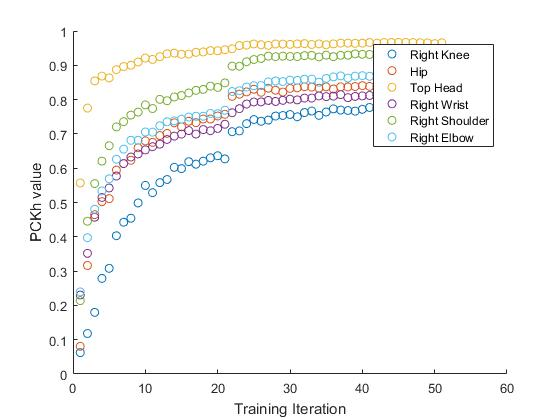
\includegraphics[width=0.8\textwidth]{pckh.jpg}
\end{figure}

\chapter{Traceability} % FILL THIS IF WE HAVE TIME
\begin{center}
\begin{longtable}{>{\raggedright\arraybackslash}p{0.2\textwidth}>{\raggedright\arraybackslash}p{0.5\textwidth}>{\raggedright\arraybackslash}p{0.4\textwidth}}
\caption{Traceability Matrix for Test-Requirement Relationships}\label{Table_TestsAndRequirements}
\\\toprule
\textbf Test Section & \textbf Description & \textbf Requirement\\\midrule
3.1.1  & Reliability and Availability of the web interface & Req \# 27, 28\\
\hline
3.2.1  & Solution Constraints and accuracy of deep learning & Req \# 1\\
\hline
3.2.2  & Solution Constraints for data rich storage  & Req \# 2\\
\hline
6.6.1  & Implementation Environment to support operating systems & Req \# 3\\
\hline
4.2  & Functional Requirement that ensures video can be processed & Req \# 7\\
\hline
4.3  & Functional Requirement for joint positioning relative to timestamps & Req \# 8\\
\hline
4.5  & Functional Requirement that each media upload has associated text & Req \# 9\\
\hline
4.6  & Functional Requirement that no false postiives are returned while searching & Req \# 7\\
\hline
5.2  & Appearance Requirement for the look and feel & Req \# 12\\
\hline
5.3  & Style Requirement to implement a minimalistic design & Req \# 13\\
\hline
5.4.1  & Ease of Use Requirement that an average user can use the website & Req \# 14\\
\hline
5.4.2  & Ease of Use Requirement for text box functionality & Req \# 16, 24\\
\hline
5.5 & Learning Requirement that a user can 'pose estimate' without prior knowledge & Req \# 17, 18\\
\hline
5.6 & Politeness and Understandability Requirement to hide the inner workings of deep learning & Req \# 20\\
\hline
5.4.2  & Ease of Use Requirement for text box functionality & Req \# 16\\
\hline
5.7  & Speed and Latency Requirement to minimize resource cost & Req \# 22, 23\\
\hline
6.1.1  & Precision and Accuracy of bone joints positioning & Req \# 25, 26\\
\hline
6.1.2  & Precision and Accuracy of the deep learning model & Req \# 1, 26\\
\hline
6.2.2  & Reliability and Availability of the web interface & Req \# 27, 28\\
\hline
6.3  & Robustness or Fault-Tolerance Requirements to handle errors within theweb interface & Req \# 29\\
\hline
6.4.1  & Capacity Requirement for multiple connections & Req \# 31\\
\hline
6.4.2  & Capacity Requirement to populate the database with images and video & Req \# 32\\
\hline
6.6.2  & Productization Requirement for multiple export types & Req \# 37\\
\bottomrule
\end{longtable}
\end{center}
\section{Modules}
Similarly, the following is a traceability table explicitly relating test cases to modules:\\
\begin{table}
\caption{Tests and Modules Relationships}
\begin{center}
\begin{tabular}{p{6cm} p{4cm}}
\hline
\textbf Test \#  & Module \\
\hline
3.1(all subsections), 3.2.1, 4.4-4.6, 5(all sections), 6.2(all subsections) - 6.4(all subsections), 6.6.2 & ASP.NET and DB \\
\hline
3.1.3, 4.3, 5.8.2, 6.1, 6.5 & TensorFlow Models \\
\hline
3.13, 3.2.2, 4.1-4.2, 5.8.2, 6.2(all subsections), 6.6.1 & Python HTTP Server\\
\hline
\end{tabular}
\end{center}
\end{table}

\chapter{Changes After testing}

The first of our major change was to the web interface. Though our testers reviewed it favourably -- there were numerous references -- but we were also given consistent criticism that an alternate colour scheme might be a slight improvement. As such we have agreed to experiment with those improvements. In addition to changing the colour scheme the layout of the website was also changed to provide a more modern approach to how the websites information was displayed.

Testing also revealed that a JavaScript application to allow continuous requests
to the HTTP server as well as utilize a mobile platform would have greater
applicability to the Guelph team. This improvement would come alongside a
function on the website to display statistics. This would help insure greater
availability. The ability to track the database live would be both useful to
the testing team as well as an entertaining aspect for the product demo.

The last major improvement provided was an improved JavaScript plugin
for drawing the skeleton on top of an image. Testing revealed that there was
flicker with the drawn skeletons, and as such, could lead to false negatives,
where a skeleton that appears inaccurate is actually just limited by our
current skeleton drawing methods.

\end{document}
